        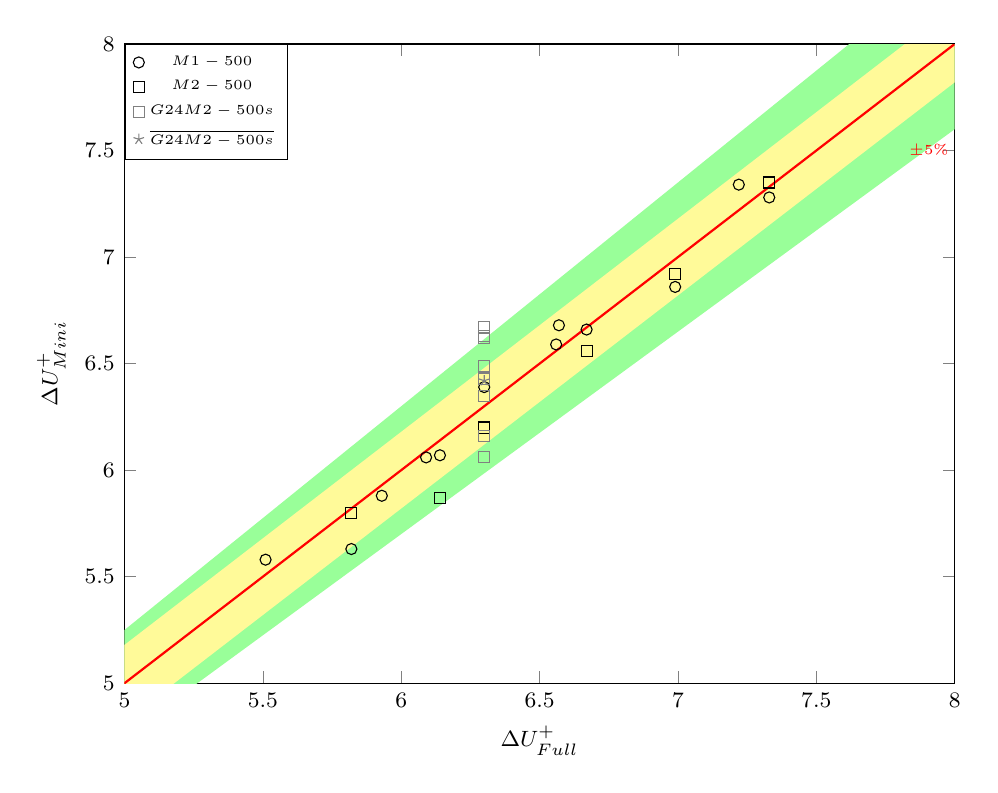
\begin{tikzpicture}[]
        \centering
        \begin{axis}[
            ylabel={$\Delta U_{Mini}^+$},
            xlabel={$\Delta U_{Full}^+$},
            ymin=5, ymax=8,
			xmax=8,
			xmin=5,
			%xtick={-2,-1.5,...,-0.4},
            width=1\linewidth,
            height=.8\linewidth,
            label style={font=\footnotesize},
			legend style={font=\tiny,at={(0,1)},anchor=north west},
            tick label style={font=\footnotesize}
            ]
			\addplot [
            black,only marks,mark=o,
            ]
            coordinates{
            (6.67, 6.66)
            (6.56, 6.59)
            (6.30,6.39)
            (5.93,5.88)
            (7.33,7.28)
            (7.22,7.34)
            (6.99,6.86)
            (6.57,6.68)
            (6.14,6.07)
            (6.09,6.06)
            (5.82,5.63)
            (5.51,5.58)
            };
			\addlegendentry{$M1-500$}
			\addplot [
            black,only marks,mark=square,
            ]
            coordinates{
            (6.67, 6.56)
            (6.30, 6.20)
            (7.33,7.35)
            (6.99,6.92)
            (6.14,5.87)
            (5.82,5.80)
            };
			\addlegendentry{$M2-500$}
						\addplot [
            gray,only marks,mark=square,
            ]
            coordinates{
            (6.30, 6.06)
            (6.30, 6.43)
            (6.30, 6.35)
            (6.30, 6.49)
            (6.30, 6.62)
            (6.30, 6.67)
            (6.30, 6.63)
            (6.30, 6.16)
            };
			\addlegendentry{$G24M2-500s$}
									\addplot [
            gray,only marks,mark=star,
            ]
            coordinates{
            (6.30, 6.42)
            };
			\addlegendentry{$\overline{G24M2-500s}$}
			 \fill[color=green!40,opacity=40] (0,0) -- (9,9.45) -- (9,8.55) -- cycle;
			 			\fill[color=yellow!40,opacity=40] (0,0.18) -- (9,9.18) -- (9,8.82) -- (0,-0.18) -- cycle;
						\addplot [
            red,thick,solid,mark=square,
            ]
            coordinates{
            (0, 0)
            (9, 9)
            };
			\node[red,right] at (axis cs: 7.8,7.5) {\tiny $\pm5\%$};
        \end{axis}
        \end{tikzpicture}